\section{Doodle Jump 2 Application Analysis by Michael}

The following research has been done for the video game application ‘Doodle Jump 2’, downloaded from the Google Play Store. The package name of the official version is ‘com.limasky.doodlejump2’. The malicious version of this game was downloaded from Koodous. The version of the app that has been researched is 1.4.7. Remarkably, the legitimate version of this application is smaller than the malicious version. The real APK being 47,8MB in size and the modified APK being 36,47MB. The legitimate application can be found on: \url{https://play.google.com/store/apps/details?id=com.limasky.doodlejump2}. The malicious version is on koodous, the link being: \url{https://koodous.com/apks/c55f01d1e6039394f09d613ffe4fcff6443e421aee737bdc058bfe753b6b0099}.
\subsection{VirusTotal summary}


\noindent\makebox[\textwidth]{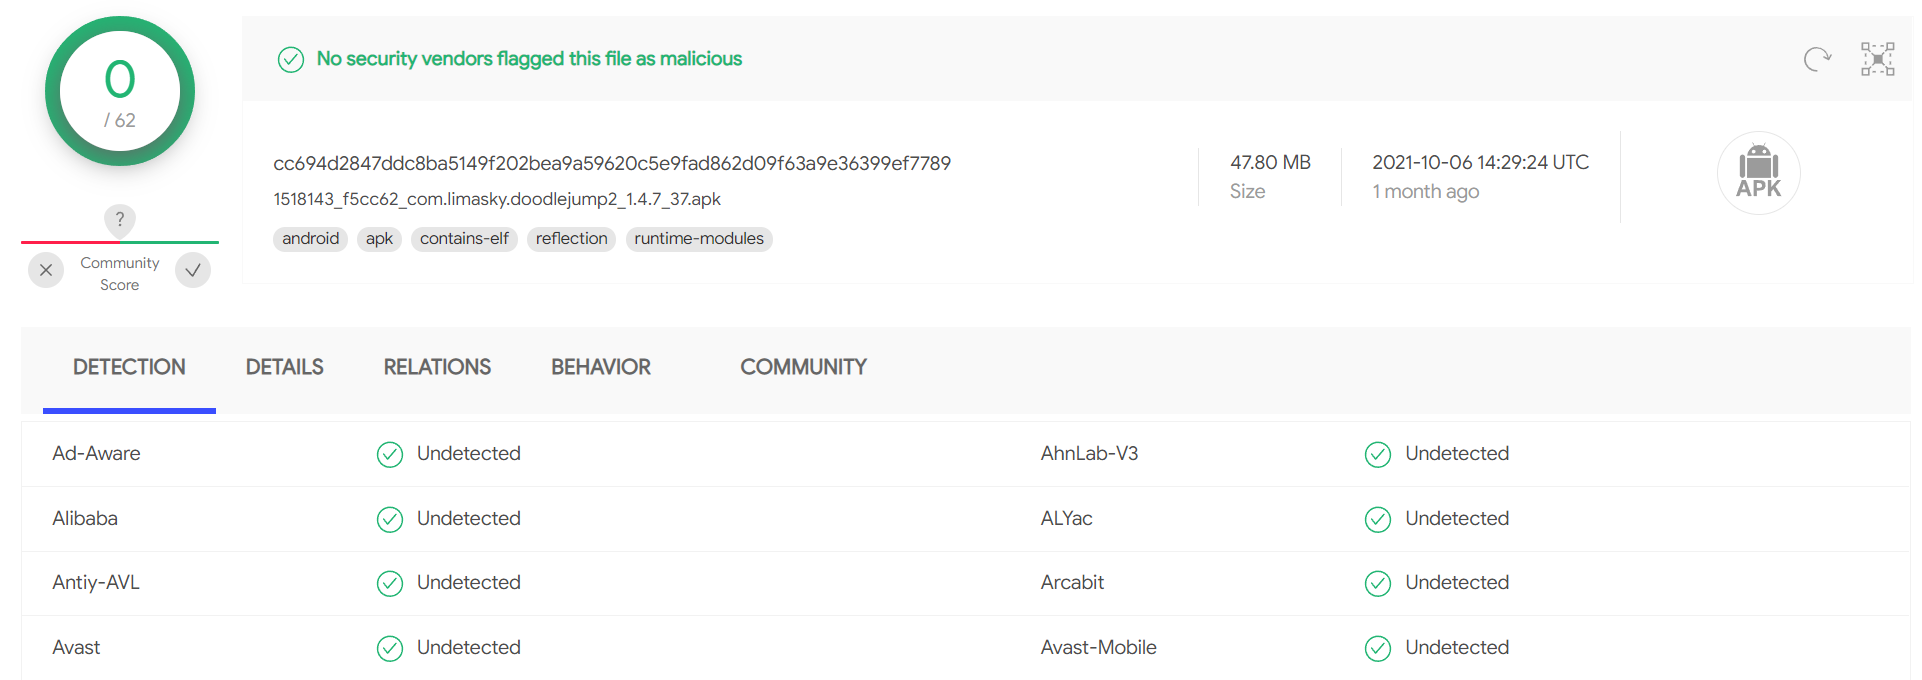
\includegraphics[width=\textwidth]{michael1.png}}

As can be seen in the above screenshot, Virustotal does not detect any kind of malicious content for the version that has been downloaded from the Google Play Store. Since this is a relatively popular app on the Google Play Store, with over 500 thousand downloads, it is safe to assume that these measurements are accurate.

\noindent\makebox[\textwidth]{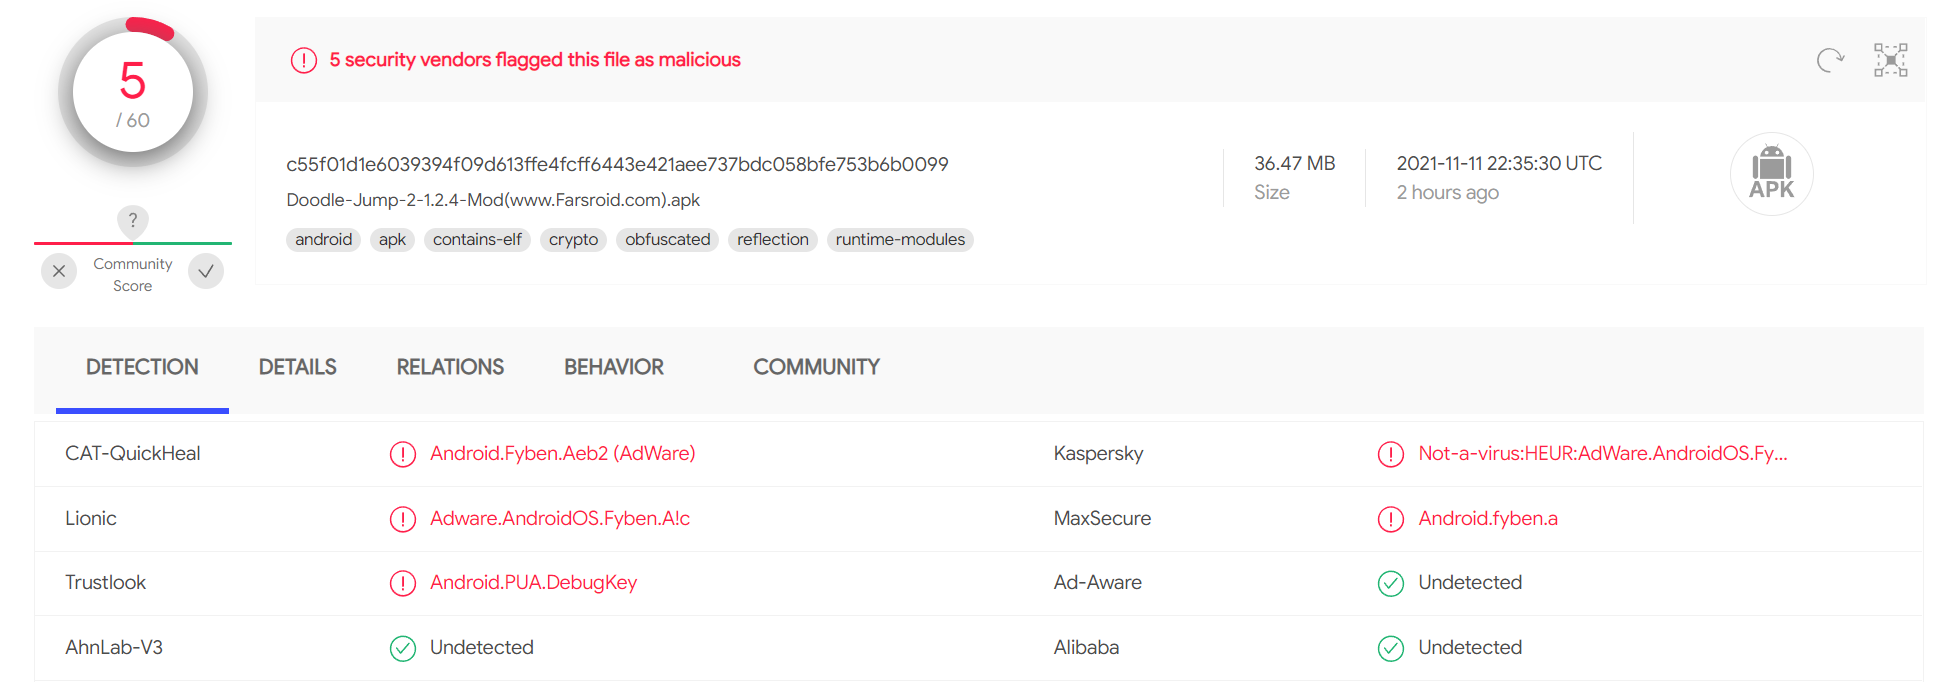
\includegraphics[width=\textwidth]{michael2.png}}

As for the Doodle Jump 2 application that I have found on Koodous, it seems this one is far more malicious than the one found on the app store. In the above screenshot it has been made clear that VirusTotal has found several issues. This APK file contains AdWare. AdWare is unwanted software that spams the user with a lot of advertisements on the screen. The attacker usually profits off of this by monetary gain. Obviously, none of the hashes match with the original version.
\subsubsection{Permission requests}

%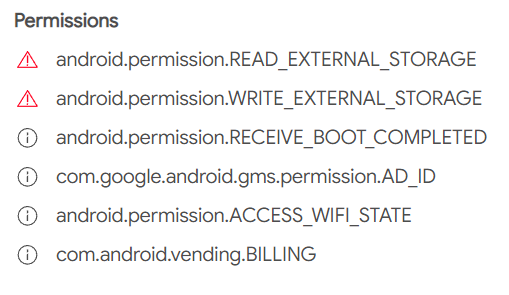
\includegraphics{michael3.png}
\begin{minipage}{\linewidth}
\begin{wrapfigure}{r}{0.5\textwidth}
\centering
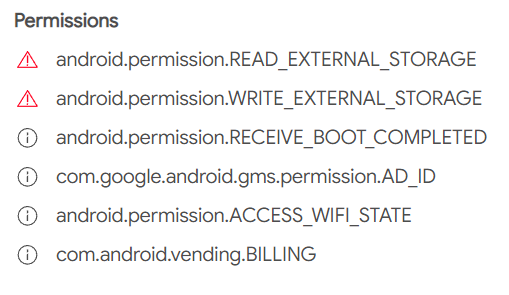
\includegraphics[scale=0.35]{michael3.png}
\end{wrapfigure}

~\\
~\\
The permissions this app requires are reasonable for a game. Reading and writing to external storage might be useful for future updates, so despite the warnings, it is still safe to assume that the app is not malicious.
\end{minipage}

~\\
~\\
~\\
~\\
~\\
~\\

%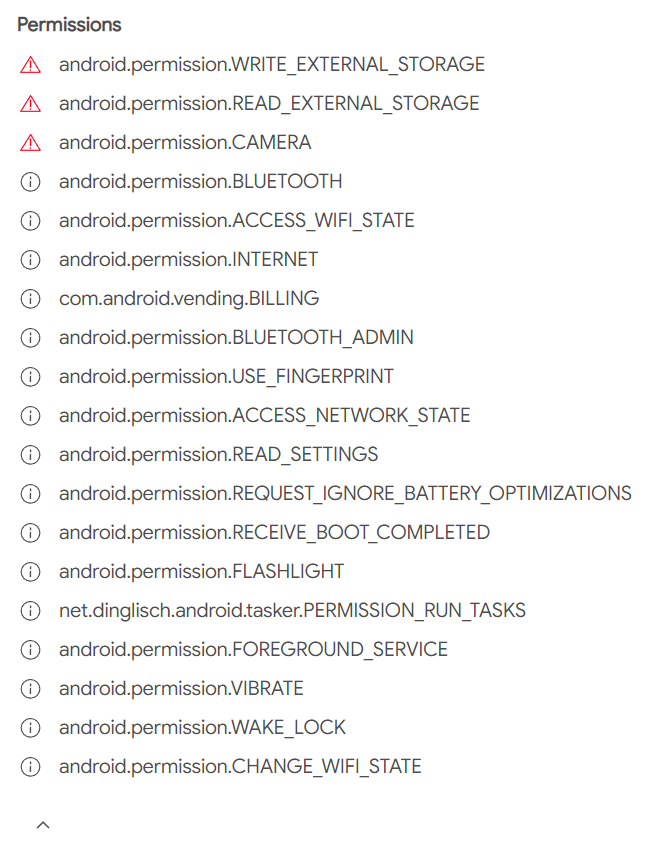
\includegraphics{michael4.png}
\begin{minipage}{\linewidth}
\begin{wrapfigure}{l}{0.55\textwidth}
\centering
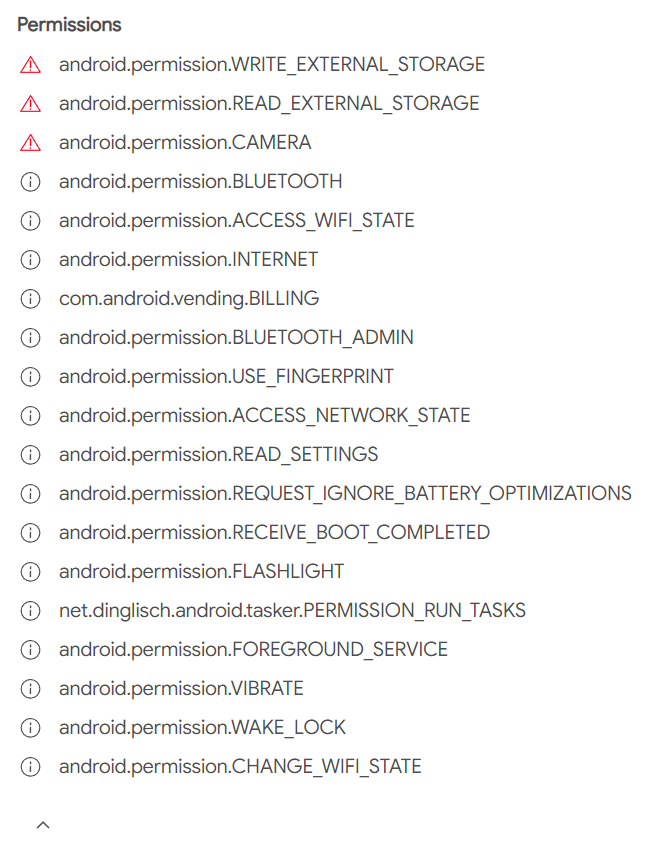
\includegraphics[scale=0.3]{michael4.png}
\end{wrapfigure}

~\\
~\\
As can be seen, a lot more permissions are required than from the official version. What these permissions are for can be read, but what they are actually being used for is unknown. Most likely for malicious activity.

\end{minipage}

\newpage
\subsection{Behavior analysis}


%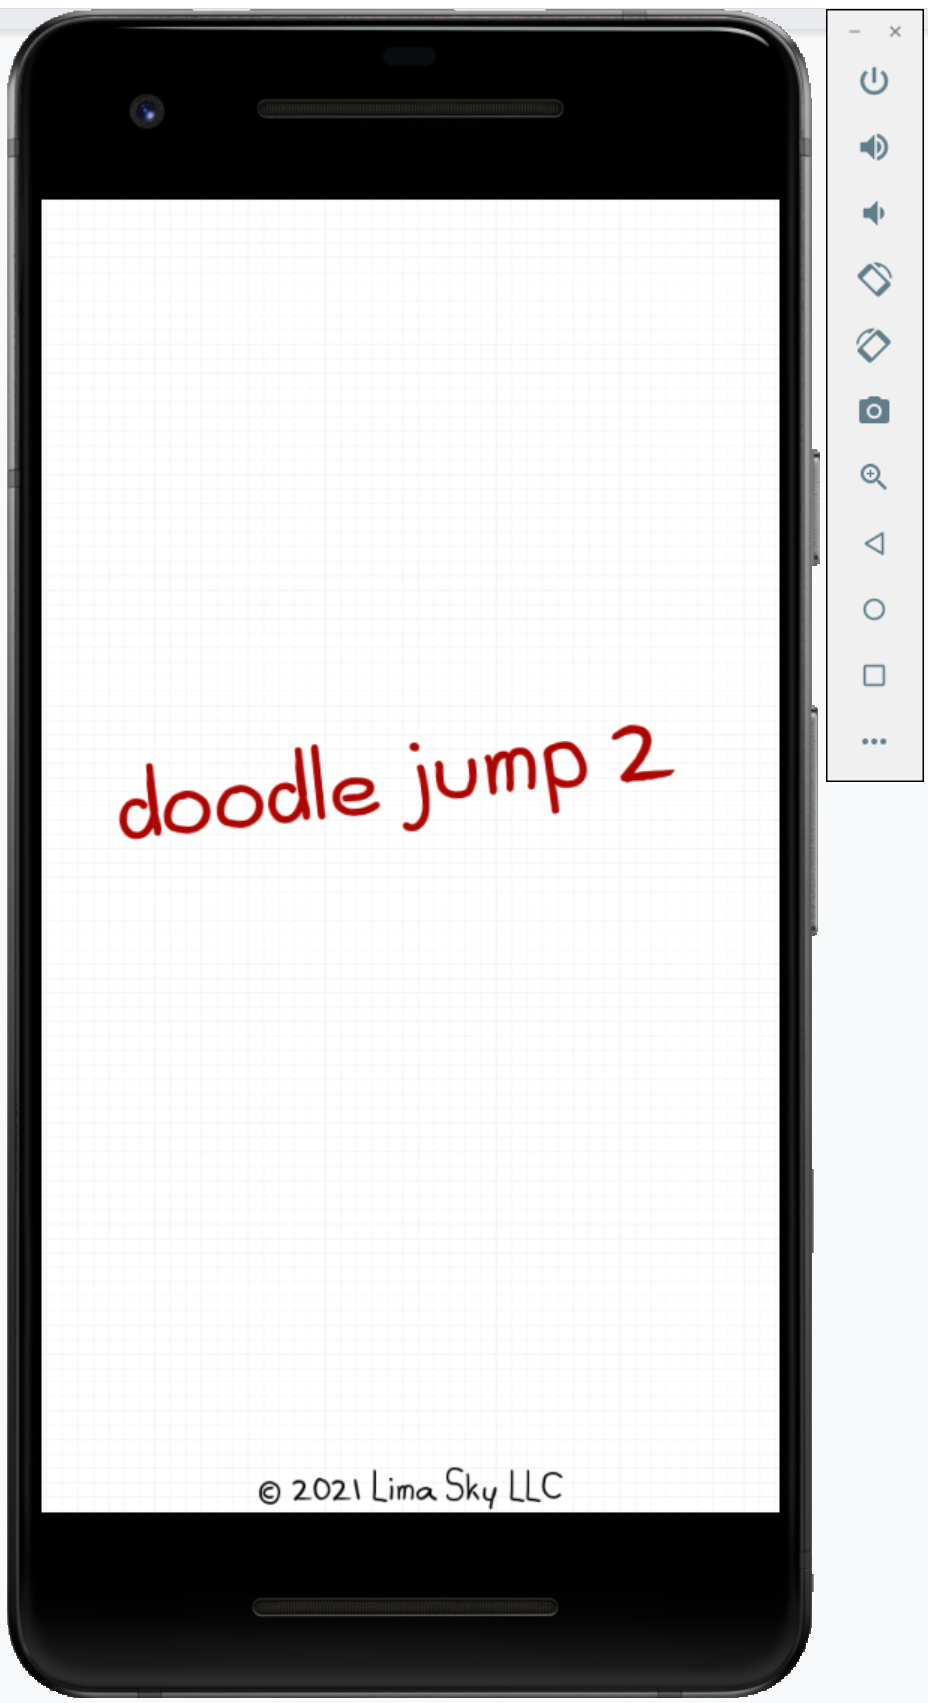
\includegraphics[width=4cm]{michael5.png}

\begin{minipage}{\linewidth}
\begin{wrapfigure}{l}{0.4\textwidth}
\centering
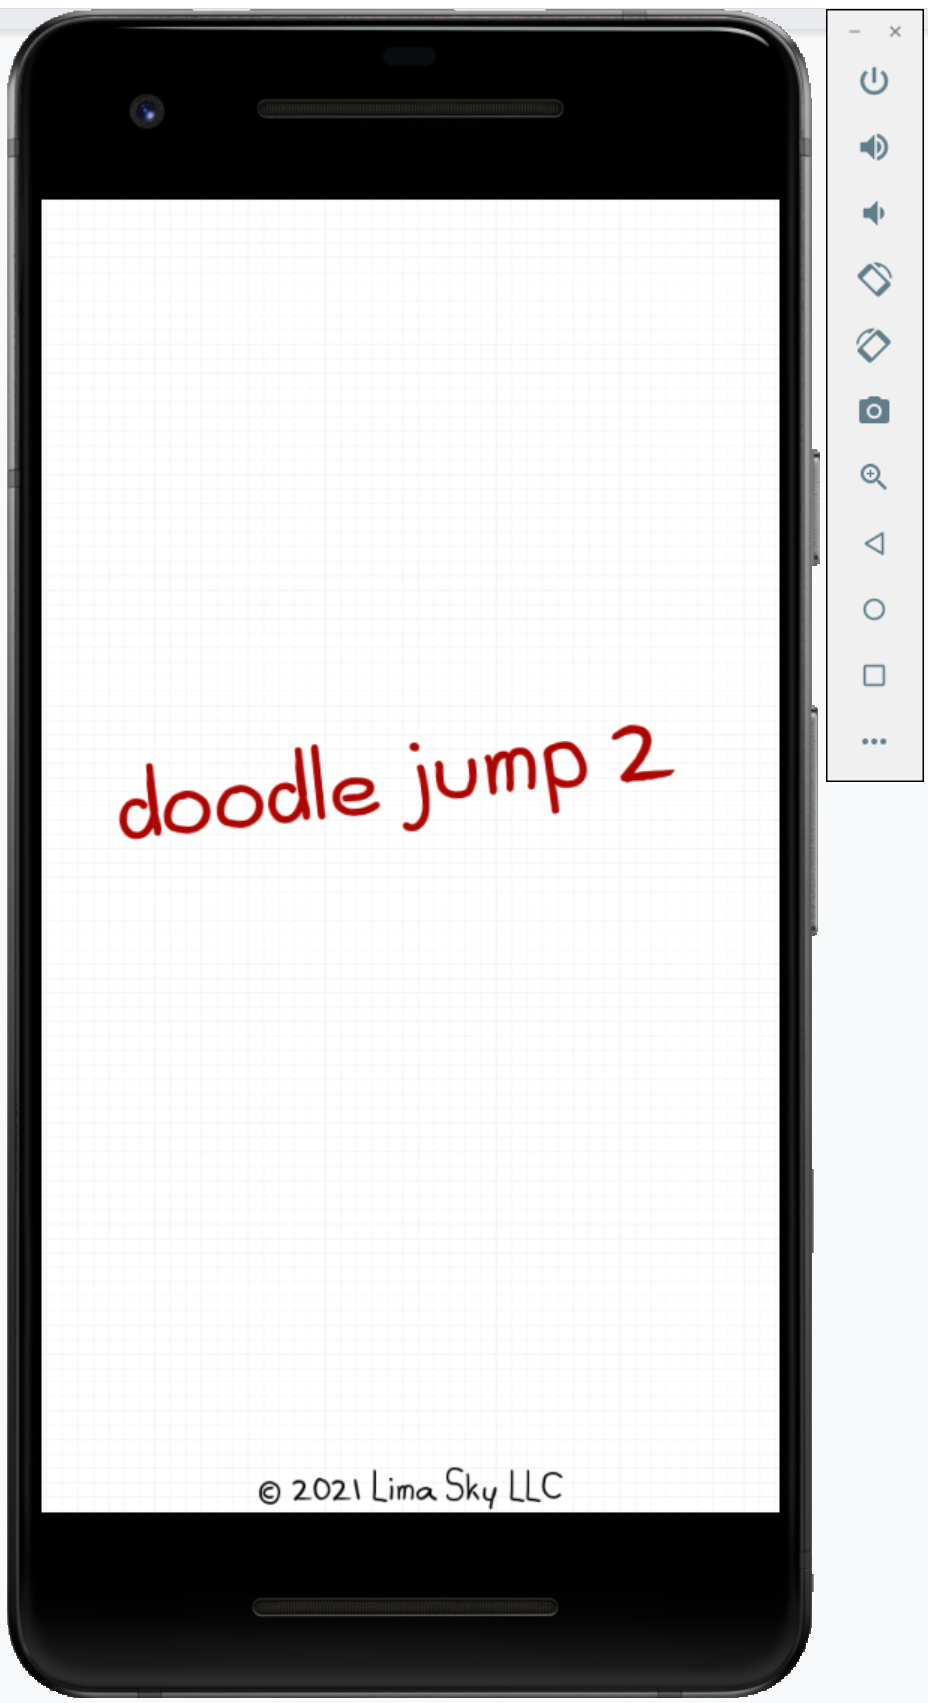
\includegraphics[scale=0.15]{michael5.png}
\end{wrapfigure}

~\\
~\\
During the installation process and gameplay of the original application, nothing out of the ordinary was found. After the installation was done the application could be found in the app drawer with its corresponding icon. Booting up the application everything worked fine. The screen, which can be seen in the screenshot above, was shown. After that it was possible to play the game starting from level one. Since this game requires tilting, it was hard to actually progress in the levels, but still it worked to some degree which made it certain that the game was running as it should.

\end{minipage}

~\\
~\\
~\\
~\\
~\\
~\\
~\\
~\\
~\\
~\\
~\\
~\\
~\\
~\\
~\\
~\\
~\\
~\\
~\\
~\\
~\\
~\\
~\\
~\\
~\\
~\\
~\\

\newpage

\begin{figure}
\centering
\begin{minipage}{.5\textwidth}
  \centering
  
\includegraphics[width=.4\linewidth]{michael6.png}
  \caption{Legitimate Application}
  \label{fig:test1}
\end{minipage}%
\begin{minipage}{.5\textwidth}
  \centering
  
\includegraphics[width=.4\linewidth]{michael7.png}
  \caption{Malicious Application}
  \label{fig:test2}
\end{minipage}
\end{figure}

As for the malware-ridden application, the installation also went smoothly. It was however necessary to uninstall the previous application, since Android thought this app to be a downgraded version of the previous one. After uninstalling the other app this one worked fine. Nothing seemed out of the ordinary until the app had actually been installed. Namely, the app icon in the app drawer for the game did not seem to match entirely with that of the original app. It is similar, however, it seems like it has been zoomed out a bit. See above for comparisons.

%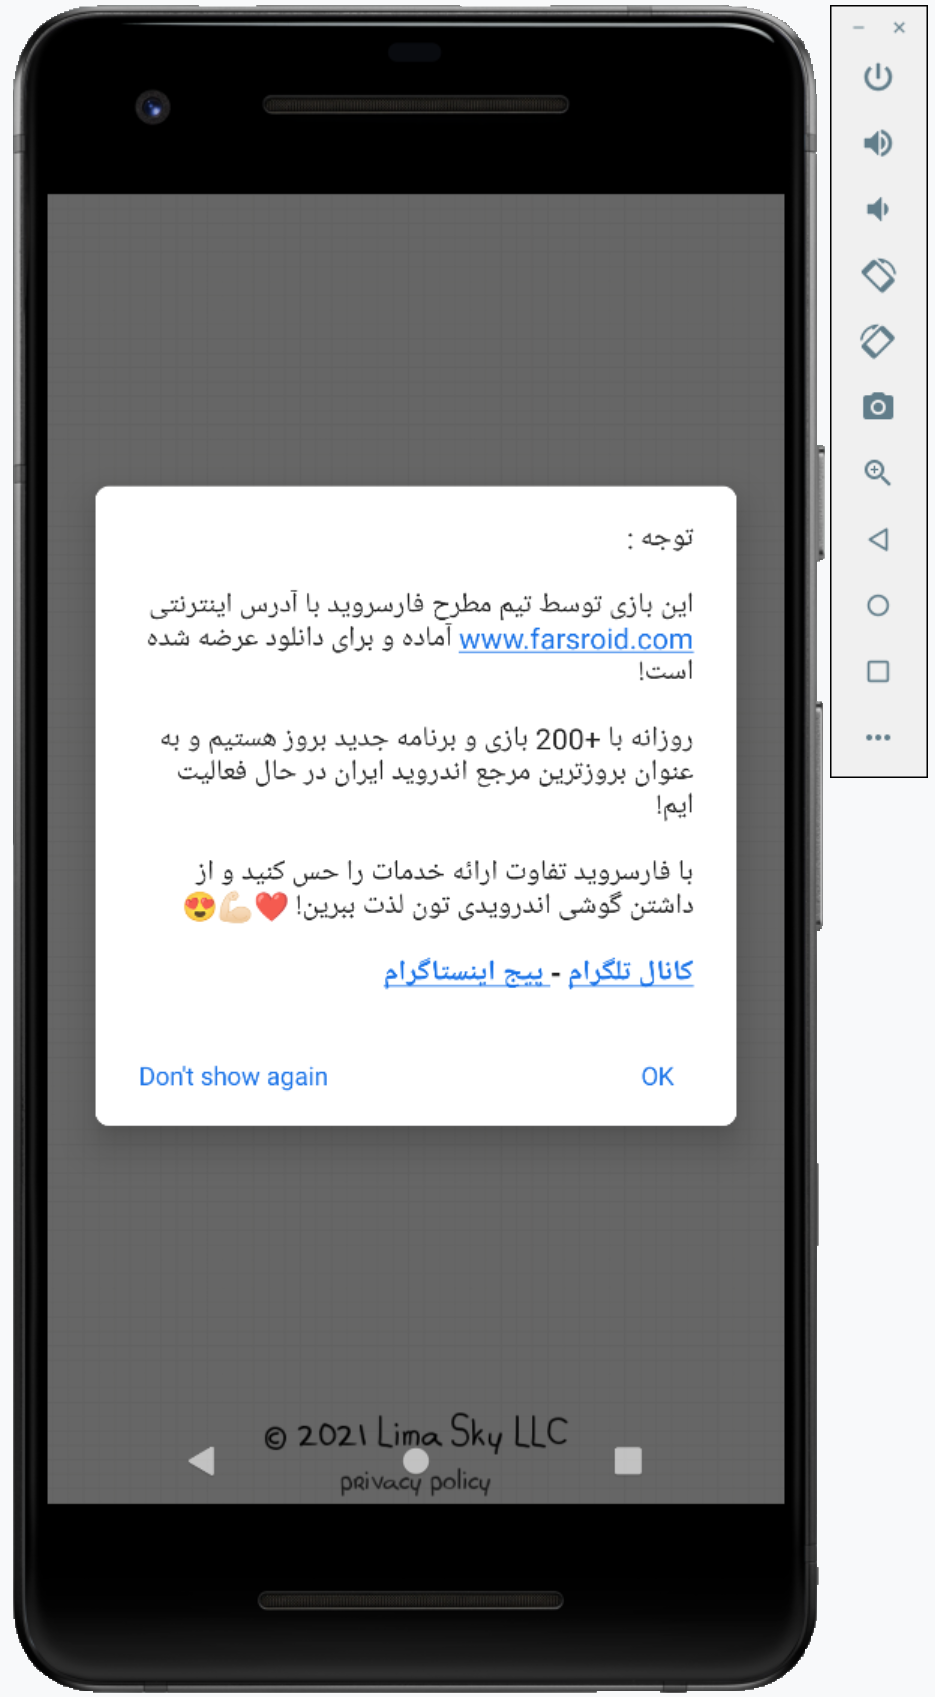
\includegraphics[width=4cm]{michael8.png}
\begin{minipage}{\linewidth}
\begin{wrapfigure}{l}{0.4\textwidth}
\centering
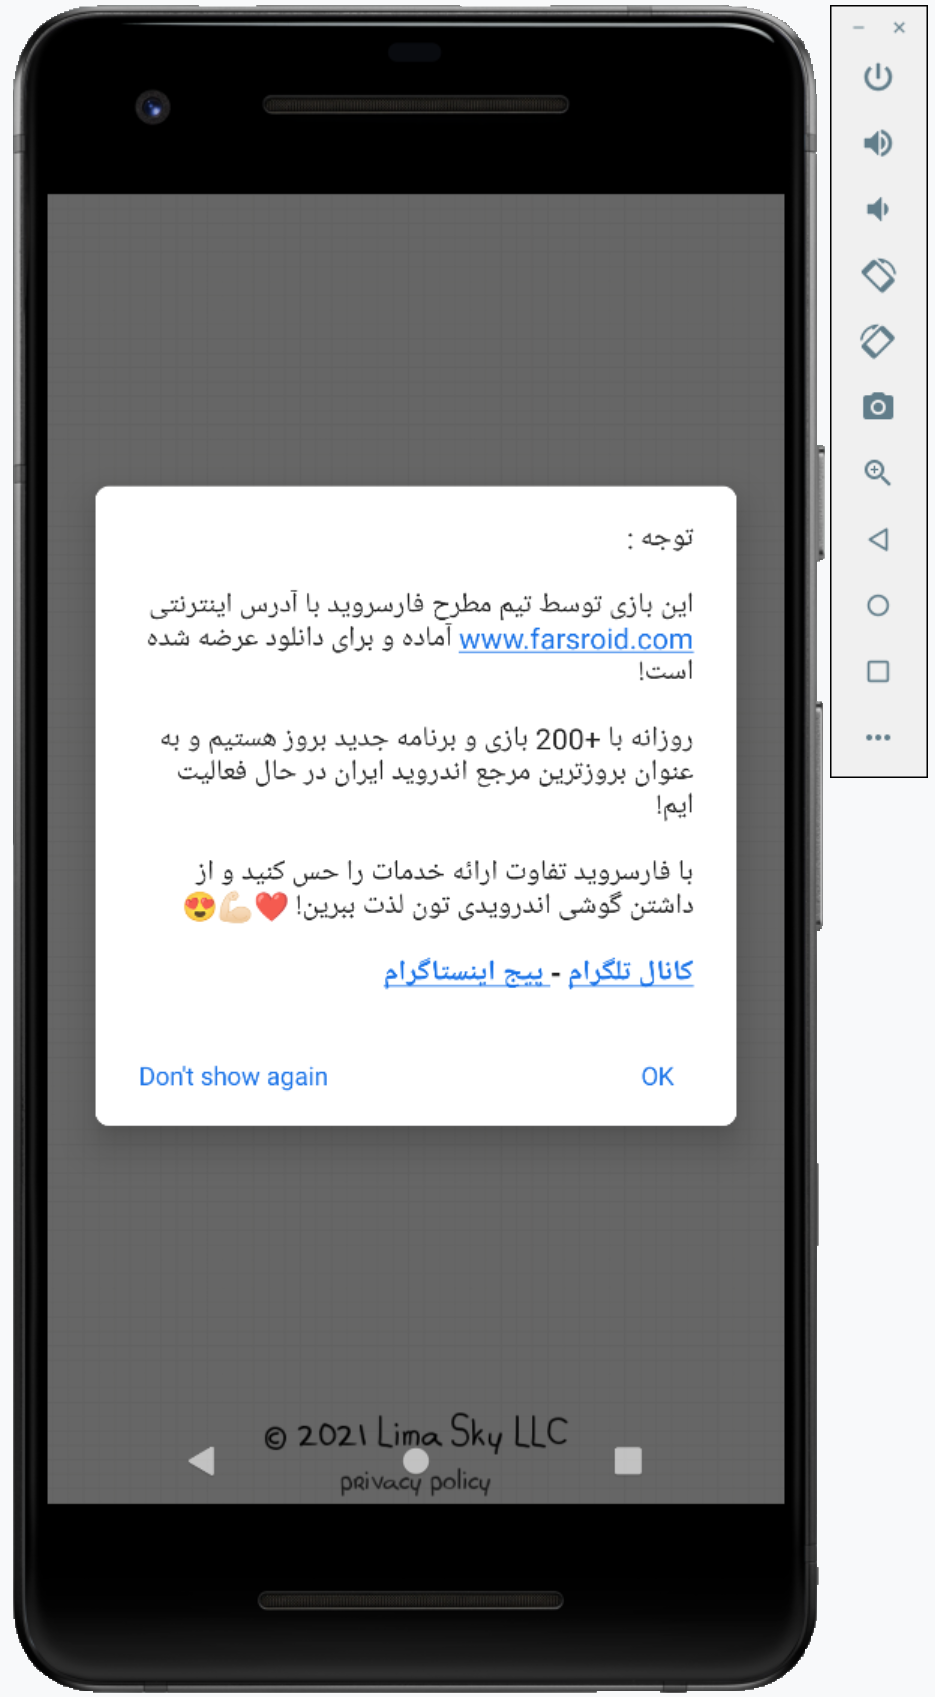
\includegraphics[scale=0.15]{michael8.png}
\end{wrapfigure}


Attempting to run the app, the user is greeted with some kind of Arabic message. The most interesting part in this message was perhaps a link to an url. It leads to a website which is also entirely in Arabic. A lot more applications could be found on this website, even some of the more known ones. It seems like the website of a hobbyist who likes to distribute modified versions of Play Store applications. Tapping either ‘Don’t show again’ or ‘OK’ on the message allows the user to get in the application, and it continues booting up like normal.\\
The first thing anyone would notice when attempting to play the game is that all the levels are unlocked from the start with extremely high scores. All in-game achievements have been cleared too, in this case stars. This seems strange, since it does not incentivize players to actually play the game. What is even more interesting is that when a player would select a level to play, the character immediately falls at a score of 21. This happens at every level. The game is thus impossible to play. The entire application or phone also feels much slower, however, a memory analysis would have to be performed to confirm this hypothesis. Shutting down the app does not cause any issue, and it is possible to boot up the application again. After rebooting the game and performing a couple more tests, it seemed like the game was finally playable. The app ran at a decent speed, and it was possible to play the levels without immediately dying. It also seemed like the player earned a higher score more quickly. Despite adware being reported in VirusTotal, other than the message when booting up, no other ads or pop ups have been found.

\end{minipage}

\newpage
\subsection{Network analysis}

\begin{center}
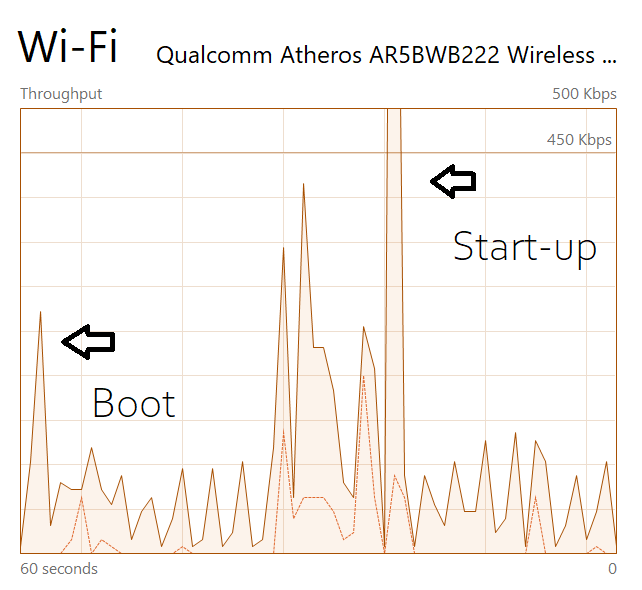
\includegraphics[scale=0.5]{michael9.png}
\end{center}

Since the graph for both the malicious, as well as the legitimate application both look the same, only one of them will be displayed. When booting up the application, there was a small spike of network usage. A possibility might be that this was when the application is connecting with the server to look for updates. This would have to be confirmed during the code analysis.
After booting up it takes a small amount of time for the application to load, after which there is a huge network spike. What this is for is as of yet unknown, but an educated guess would be to load scores for levels. Also this would have to be confirmed during the code analysis.
\subsubsection{HTTP proxy analysis}
The two captures that have been made were done so after the app was booted and initialized. The first one is for the legitimate application and the second one is for the malicious application. At first glance they don’t seem different from each other, however there are some inconsistencies.

\noindent{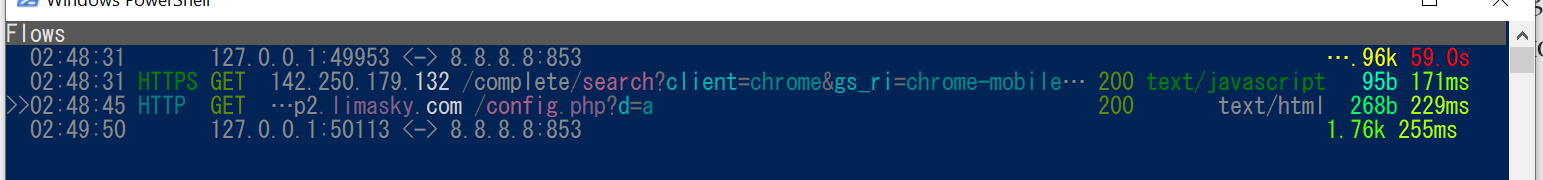
\includegraphics[width=\textwidth]{michael10.png}

The above screenshot was the output of mitmproxy for the legitimate application. Nothing seems out of the ordinary. There was a GET request for google, most likely an Android service in the background. Other than that there was a GET request for a config.php file towards the Limasky servers, which are the developers of the app. This one was not encrypted, it was a simple HTTP request. The contents, however, are not interesting.

\noindent{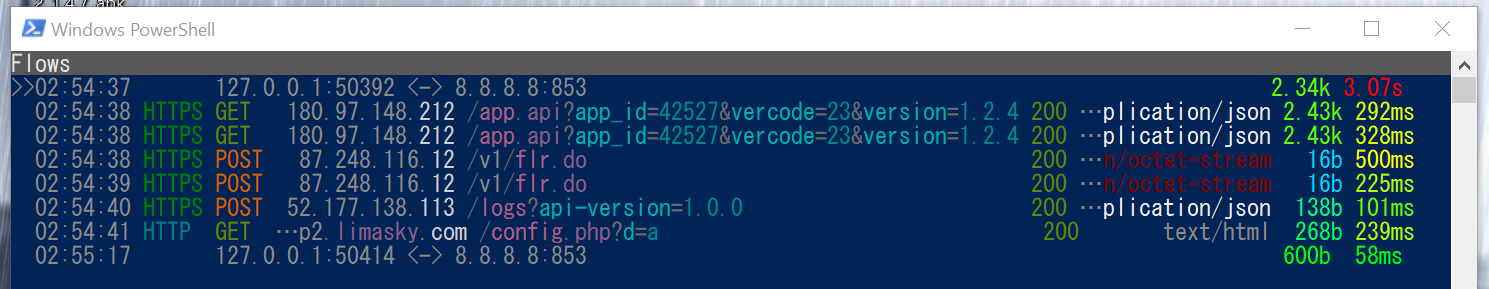
\includegraphics[width=\textwidth]{michael11.png}

This capture seems to have two GET requests and three POST requests that have to do with some kind of API. The three IP addresses associated with these requests are from huge internet companies, such as Microsoft Azure and Yahoo! UK. From this it is clear that these are thus not relevant, and are the result of a background process. Other than that, the same GET request to the Limasky servers had been made.
\subsubsection{Wireshark analysis}

\noindent{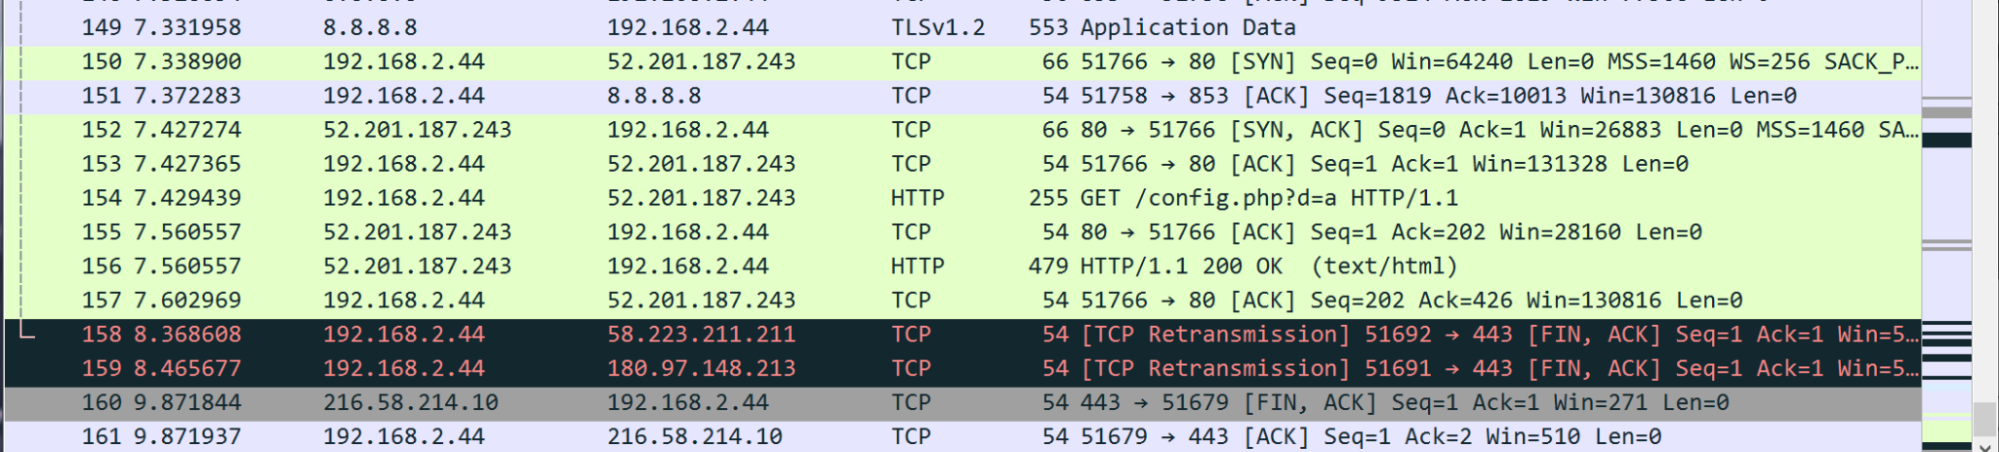
\includegraphics[width=\textwidth]{michael12.png}

For the Wireshark analysis, the malicious app was tested first. Interestingly, during start-up a TCP handshake was being performed. Other than this data there is nothing else that might be relevant. A scan has been performed on the IP address, and from this scan it became apparent that the IP is hosted by Amazon Web Services in the United States of America. This was surprising, considering malicious activity more than likely gets removed sooner or later from big hosting companies such as these. However, what happened next would subdue all suspicion one could have.

\noindent{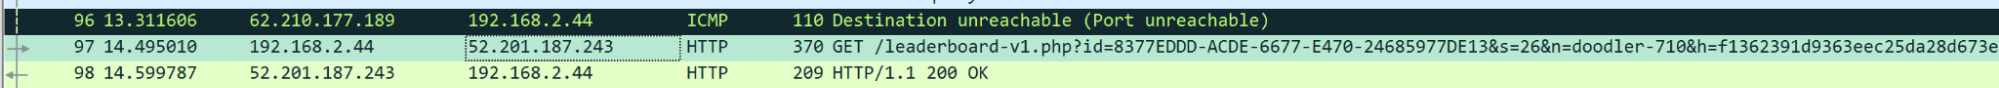
\includegraphics[width=\textwidth]{michael13.png}

The application was allowed to continue to run, and when this happened, a GET request was made to the exact same IP as before. This could only mean that this packet could only go to the legitimate source of the application. This is disappointing, but enlightening at the same time, since it is now clear that this application is not being used for harmful or malicious purposes. To confirm this hypothesis, the legitimate application was executed and tested with Wireshark and showed the exact same output as the malicious version. This means there is no malicious network traffic being found. This analysis does confirm what happened during the general network analysis, that for both applications the same amount of network traffic is being transmitted.
\subsubsection{Reconnaissance}

Using shodan.io, much of the information on the network analysis part of the research could be found. For the IP’s that had significance, shodan.io was used. This way it was also possible to identify what kind of hard services were provided on those networks, which in turn cleared up the picture as for what these connections were used for.

\newpage
\subsection{Code analysis}
To analyze the code of the applications, it was necessary to decompile them using a program called JadX. After this was done, Dex2Jar was used to confirm the process was completed successfully.

%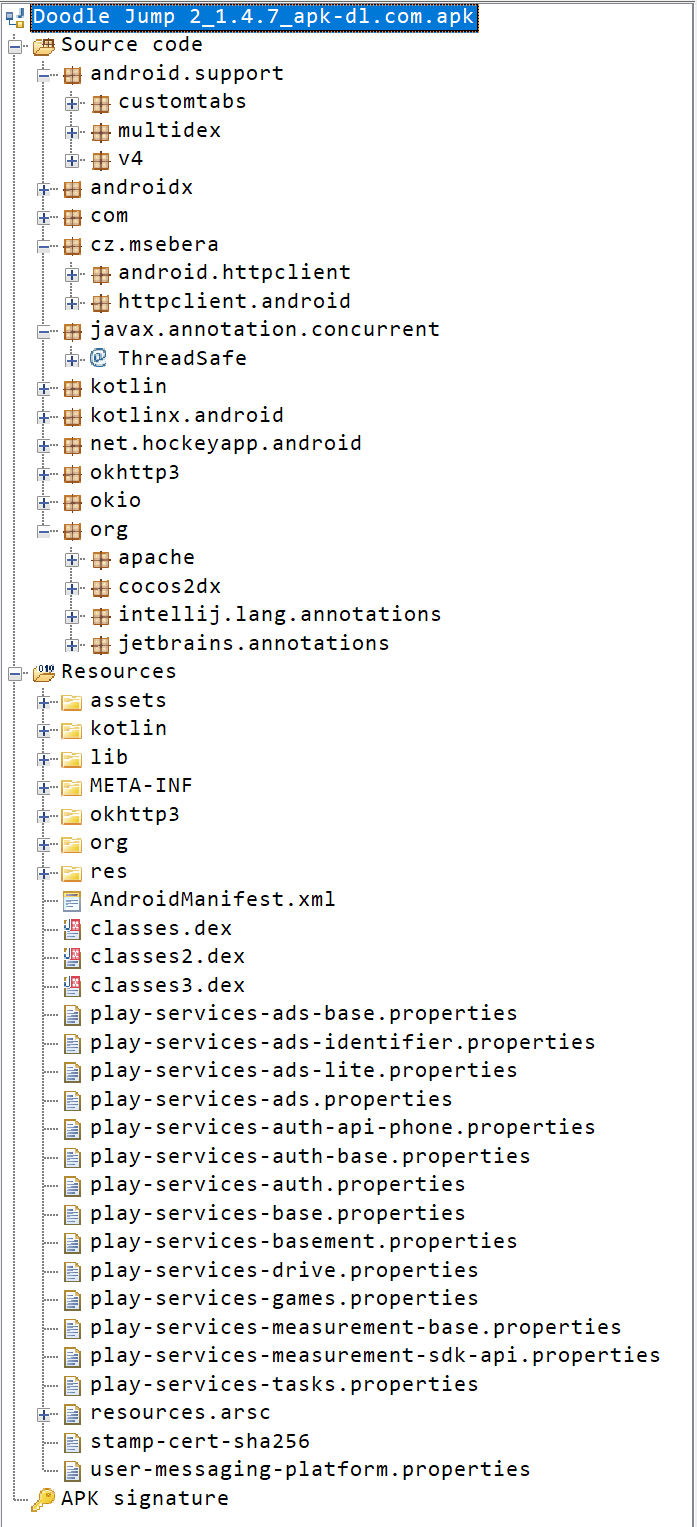
\includegraphics[width=4cm]{michael14.png}
%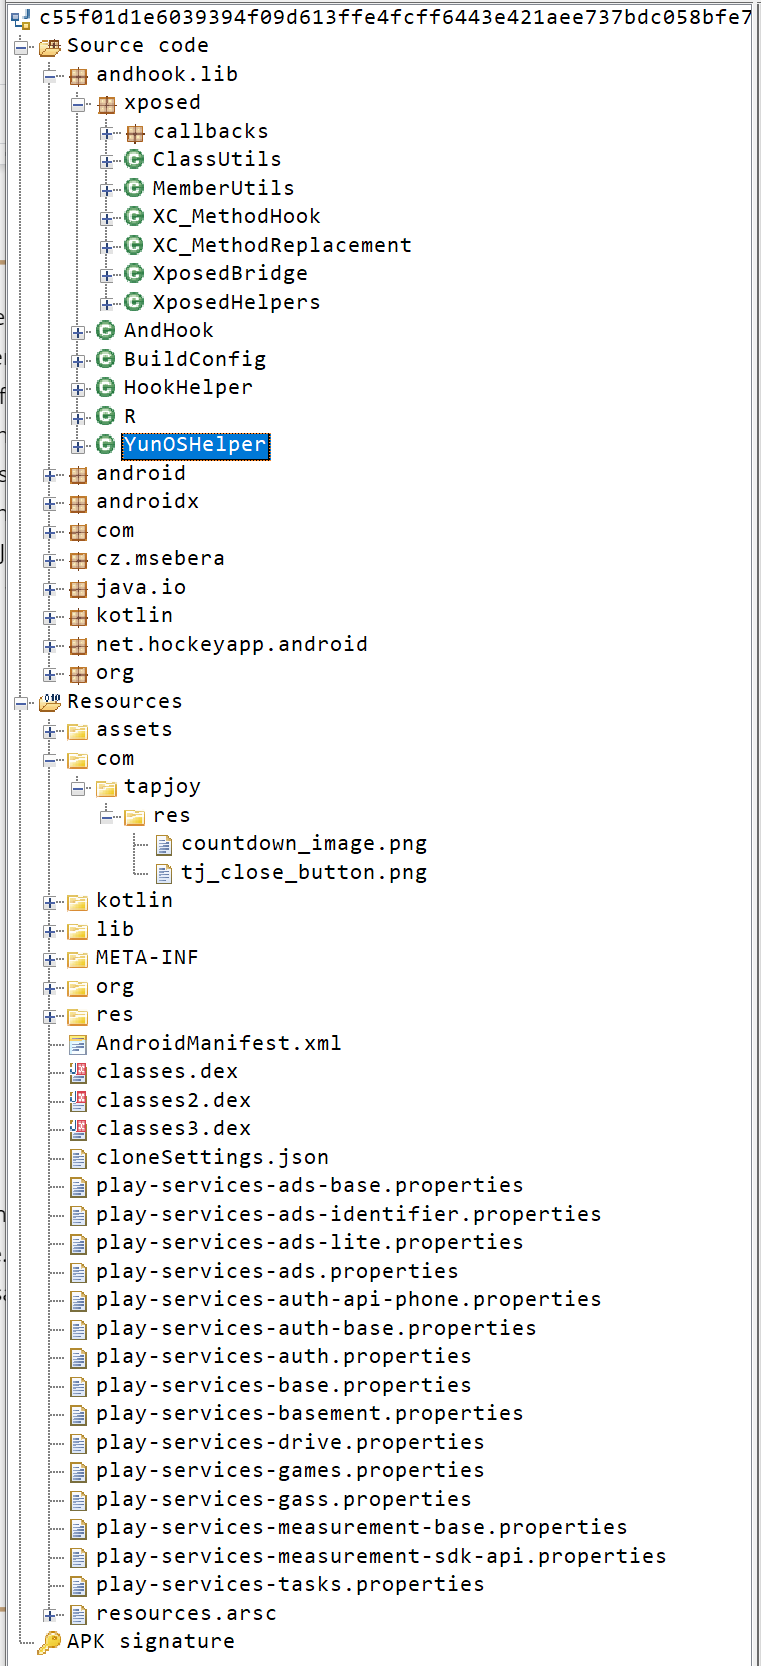
\includegraphics[width=4cm]{michael15.png}

\begin{figure}
\centering
\begin{minipage}{.5\textwidth}
  \centering
  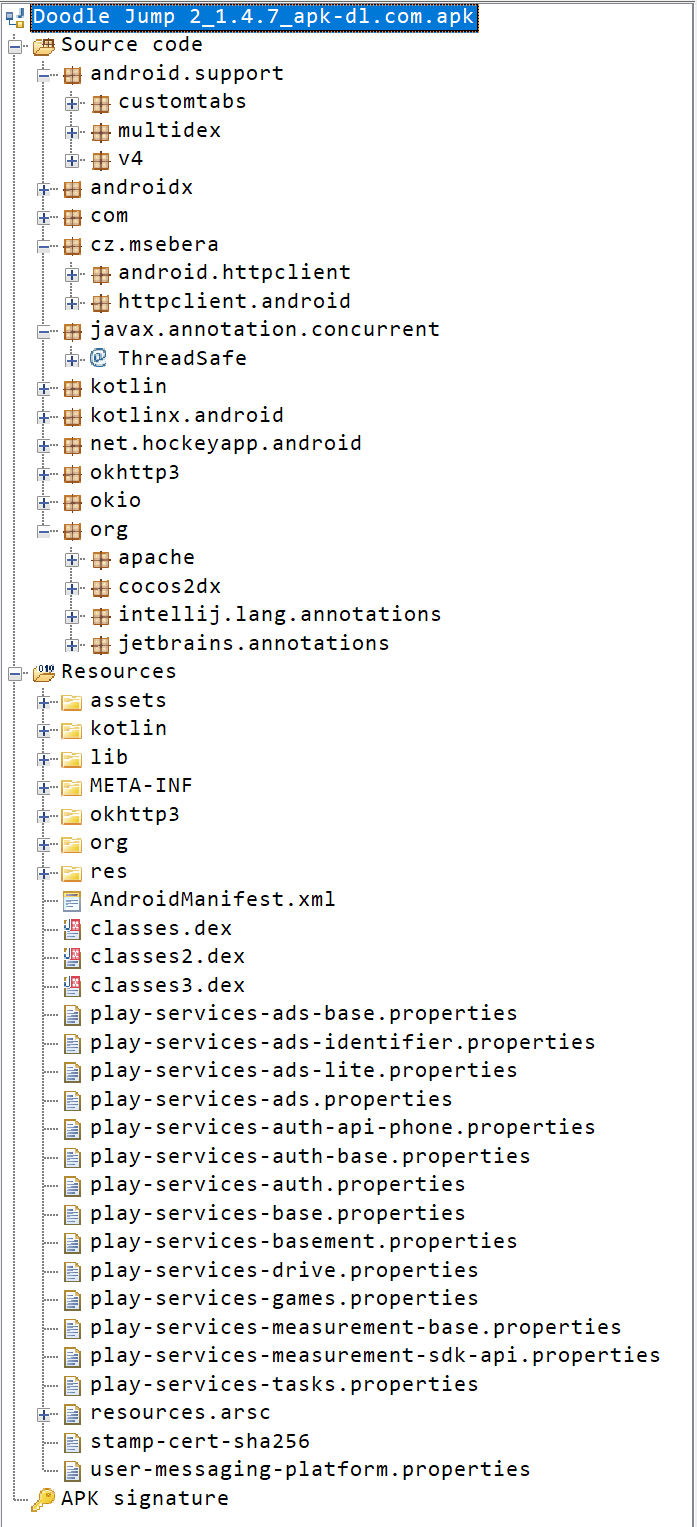
\includegraphics[width=.6\linewidth]{michael14.png}
  \caption{Legitimate Application}
  \label{fig:test1}
\end{minipage}%
\begin{minipage}{.5\textwidth}
  \centering
  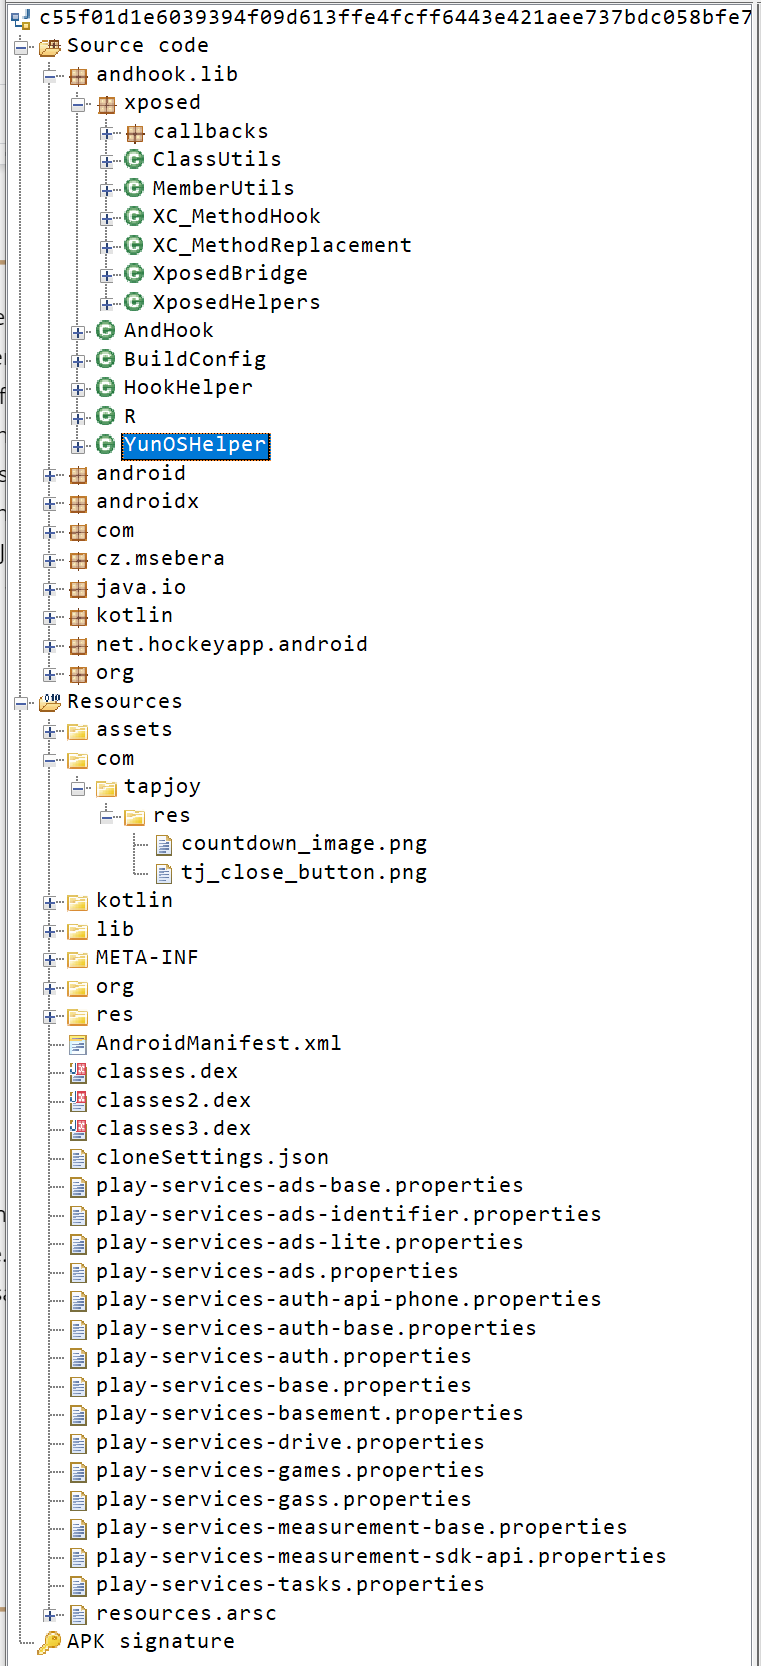
\includegraphics[width=.6\linewidth]{michael15.png}
  \caption{Malicious Application}
  \label{fig:test2}
\end{minipage}
\end{figure}

As for the source code, nothing out of the ordinary has been found. After going through the folders the usual files and folders to be included for a video game, such as a MathKt class and assets folder, were present. It is also safe to assume that the application has been written in Java on the IntelliJ IDEA development environment by JetBrains, since there were packages for development on that editor.

For the malicious version, the first thing anyone would notice is the absence of a couple of folders compared to the legitimate application, and the presence of new ones. There is now an andhook.lib library in the source code. What this does is not entirely clear and requires a higher level of understanding of game programming. Another folder I have noticed appearing is the ‘com’ folder in resources. This folder contains an image for some kind of countdown, and another for a close button. Since AdWare has been found, one would assume that these images are being used for pop-up ads which users are able to close once the countdown is over. However, during the behavior analysis, no such behaviour has been detected.

\newpage
\subsection{Process analysis}
For the memory analysis, a reliable tool, named Simple System Monitor was used. This is a popular app on the Play Store to track the usage of the CPU and RAM. However, the CPU details could not be recorded since the device is emulated. This is highly unfortunate, but at least it is possible to note the RAM usage.

%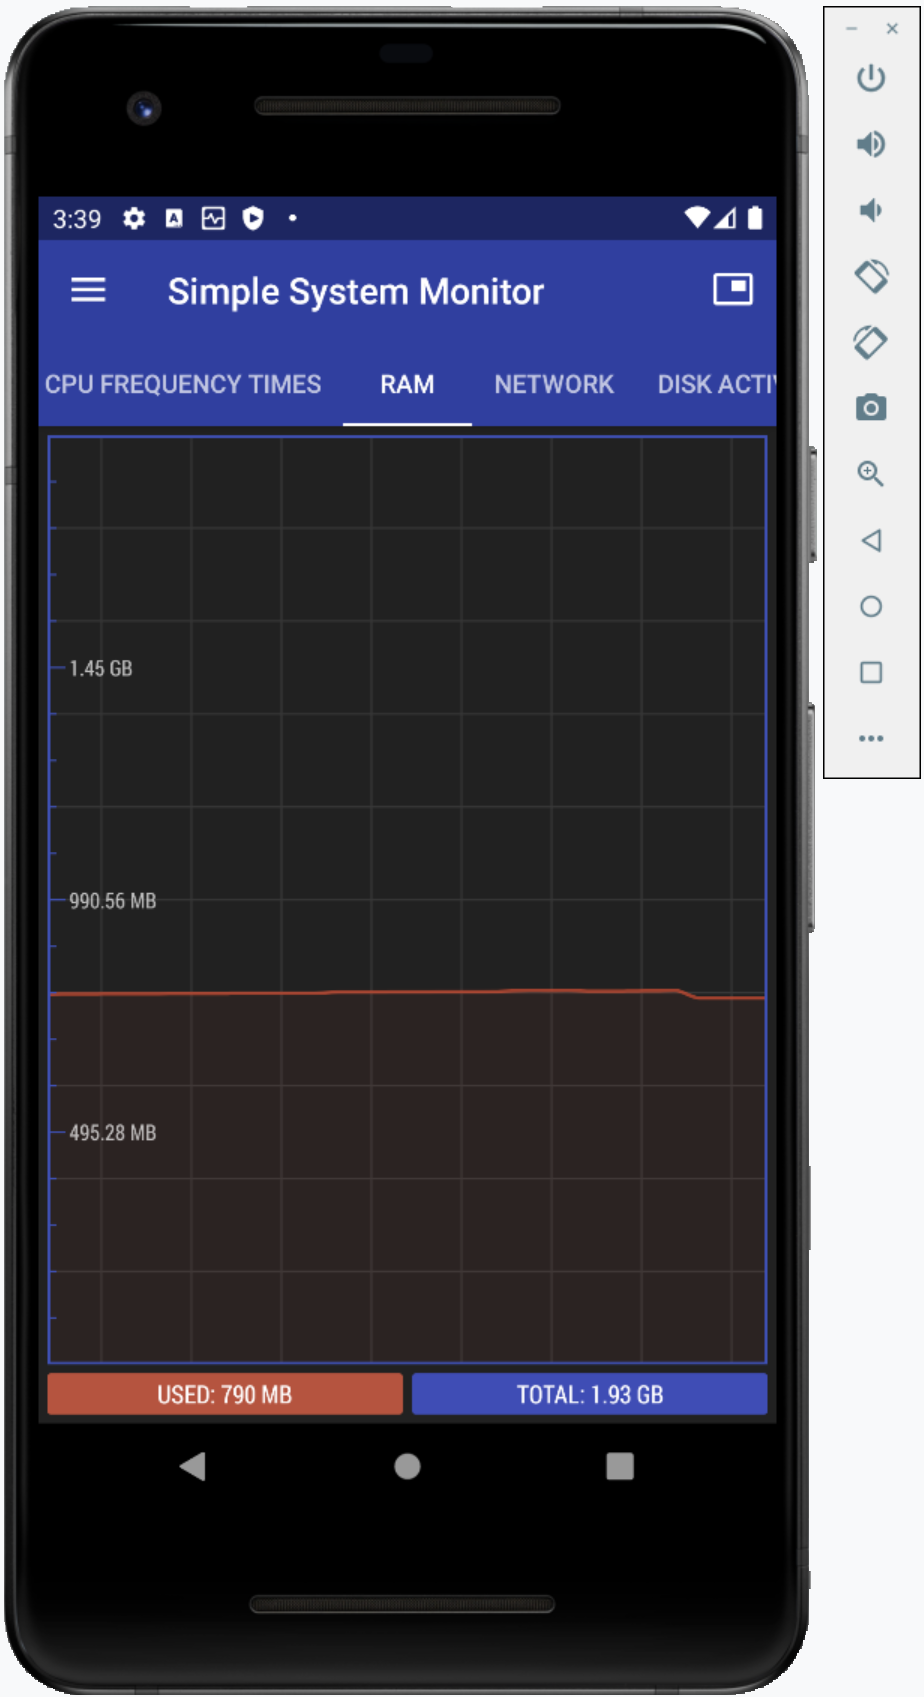
\includegraphics[width=4cm]{michael16.png}
\begin{minipage}{\linewidth}
\begin{wrapfigure}{l}{0.4\textwidth}
\centering
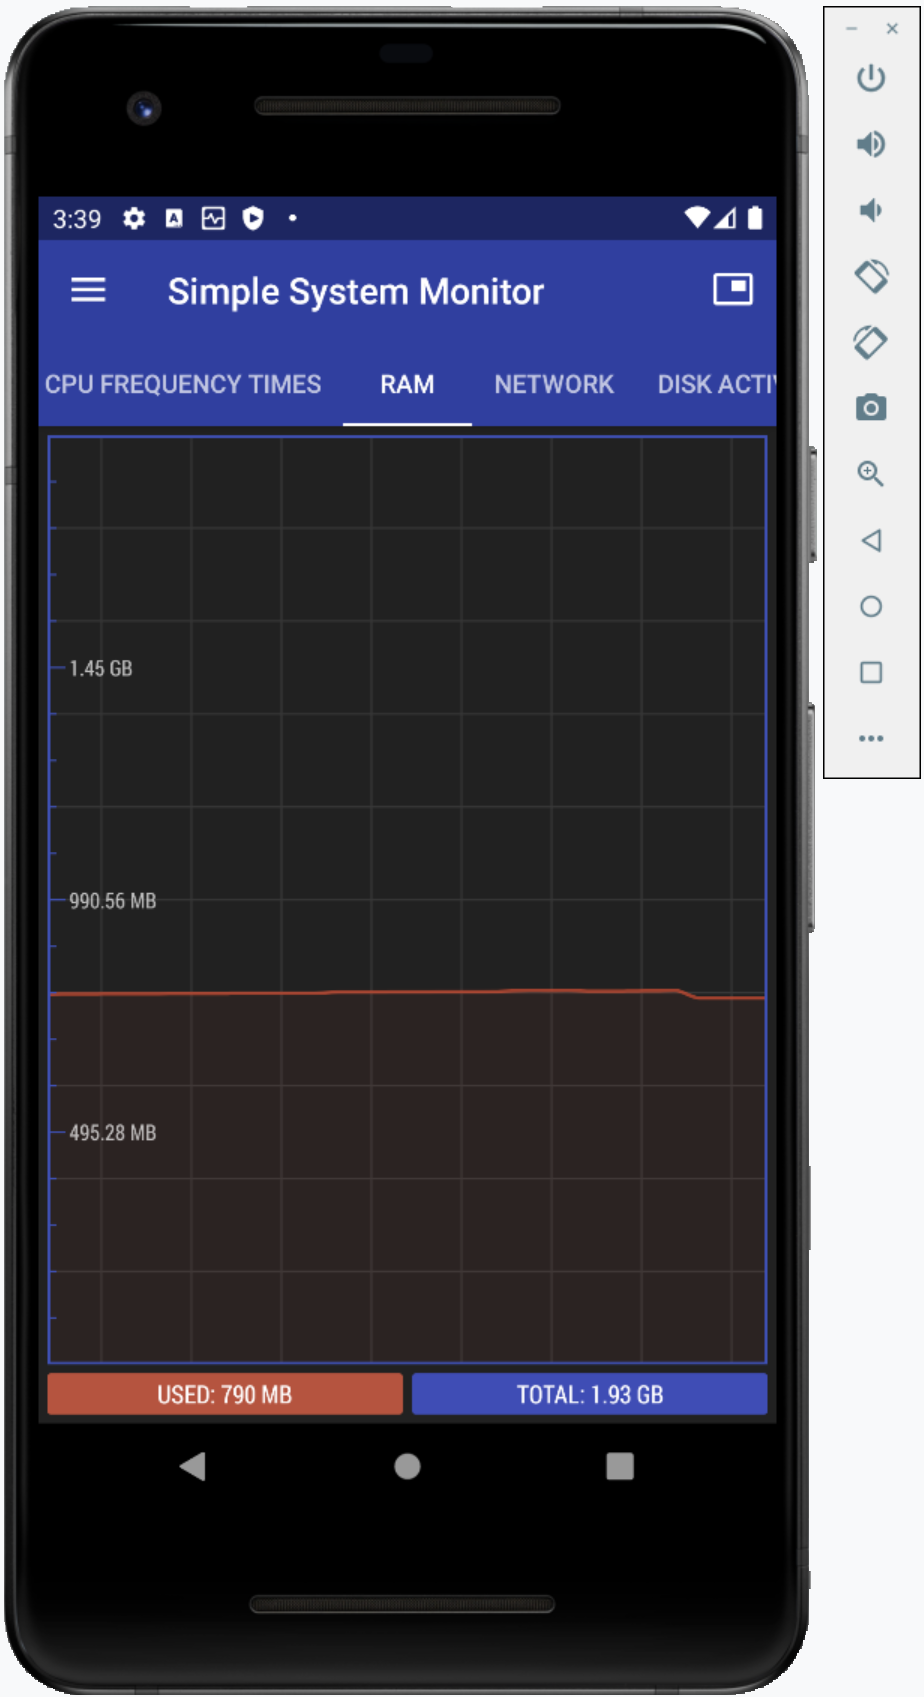
\includegraphics[scale=0.15]{michael16.png}
\end{wrapfigure}
~\\
~\\
~\\
~\\
~\\
~\\
~\\

This was the RAM usage while idle. As can be seen, it consists of a stable 790MB of data used. This was most likely being used by native Android processes, since no other processes are currently running.
\end{minipage}
~\\
~\\
~\\
~\\
~\\
~\\
~\\
~\\
~\\
~\\
~\\
~\\
~\\

%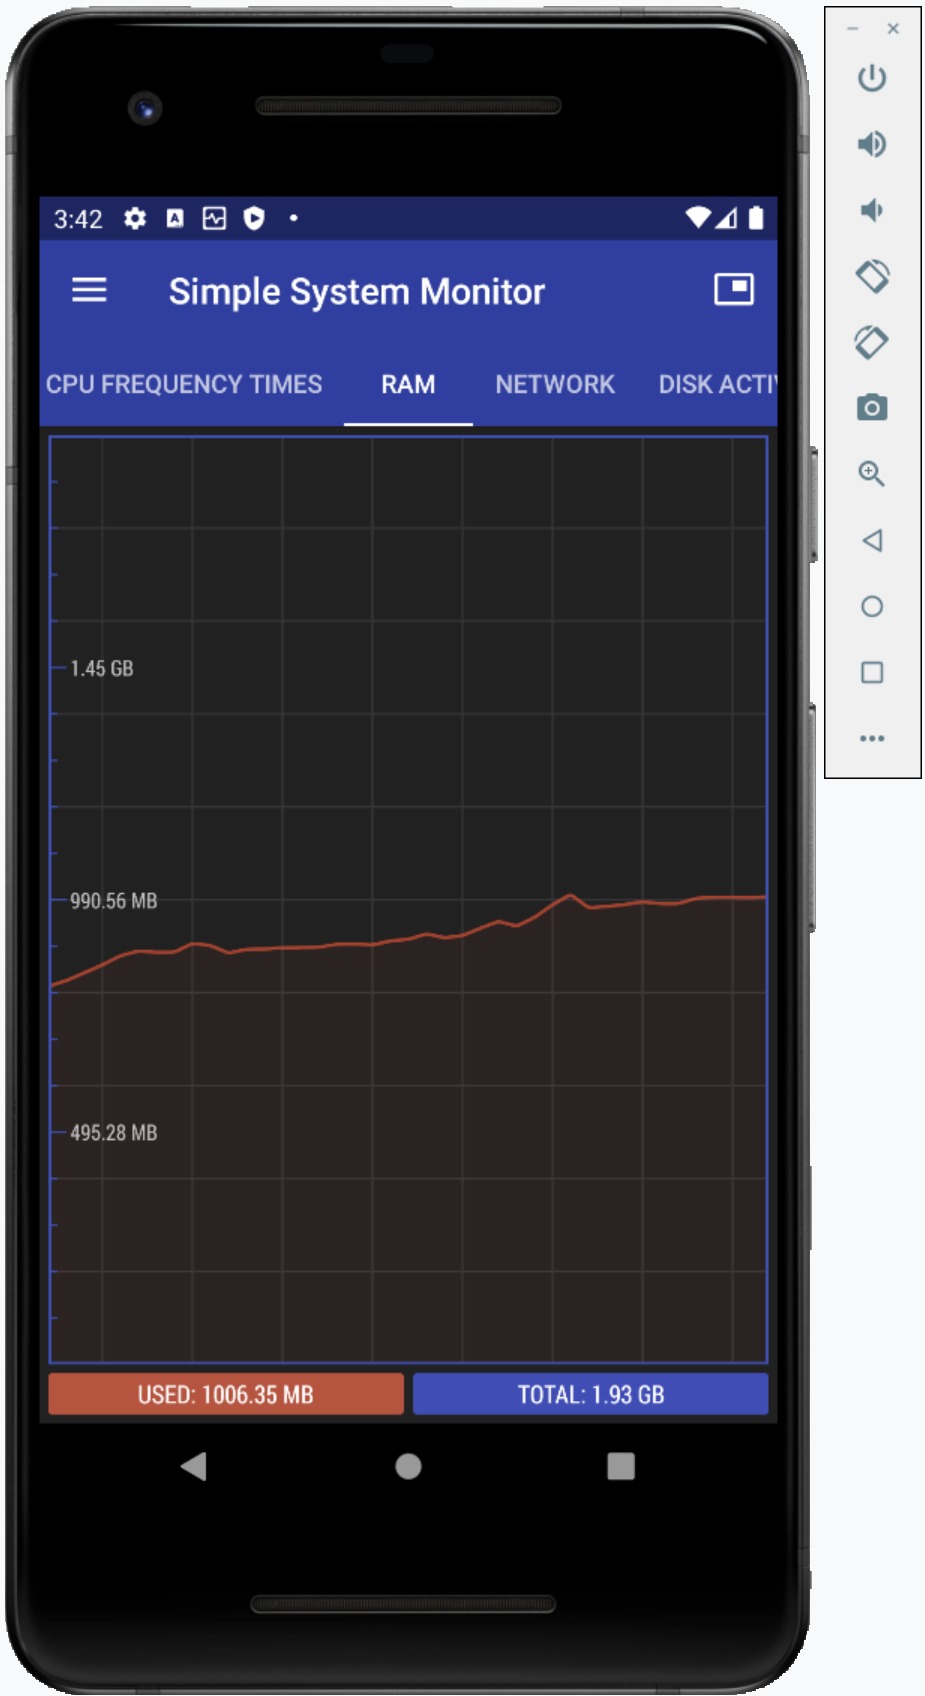
\includegraphics[width=4cm]{michael17.png}
\begin{minipage}{\linewidth}
\begin{wrapfigure}{r}{0.4\textwidth}
\centering
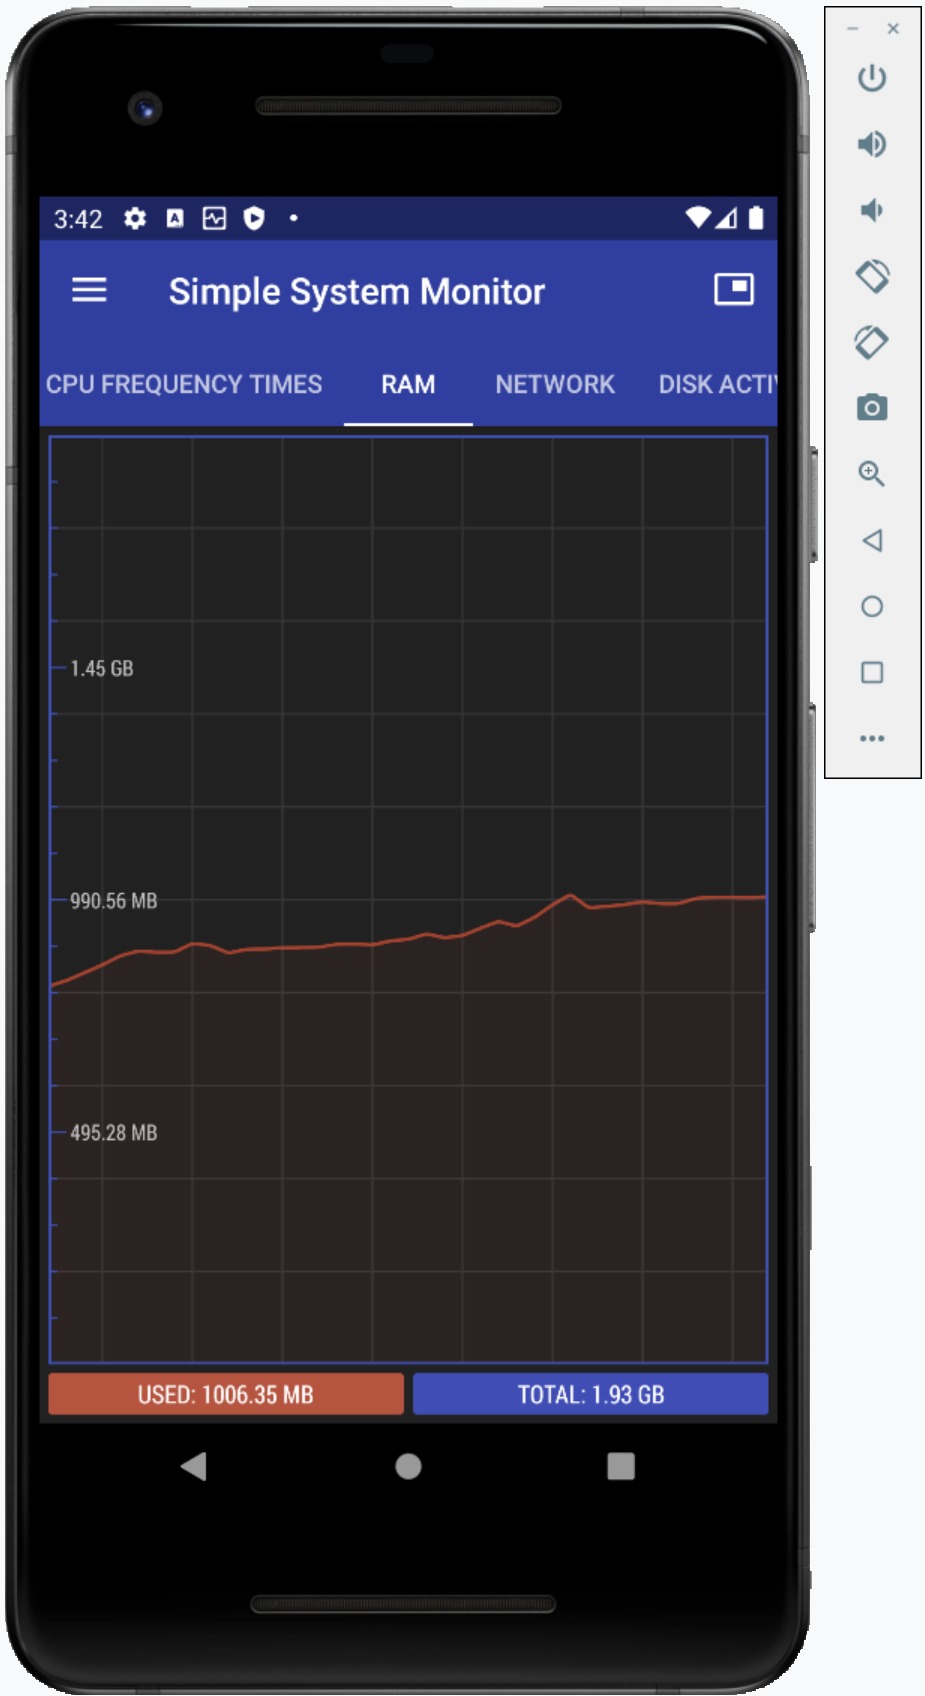
\includegraphics[scale=0.15]{michael17.png}
\end{wrapfigure}
~\\
~\\
~\\
~\\
~\\
~\\
~\\

Running the legitimate application until user interaction was possible, which is to say after boot-up and loading time, another screenshot has been made of the used RAM. The used memory shot up to more or less 1006MB of data. This means that the application used about 215MB of data. This is ordinary for an application such as this. Shutting down the application the used RAM went back down to about 820MB. This most likely consists of cached data.
\end{minipage}
~\\
~\\
~\\
~\\
~\\
~\\
~\\
~\\
~\\
~\\
~\\
~\\
~\\

%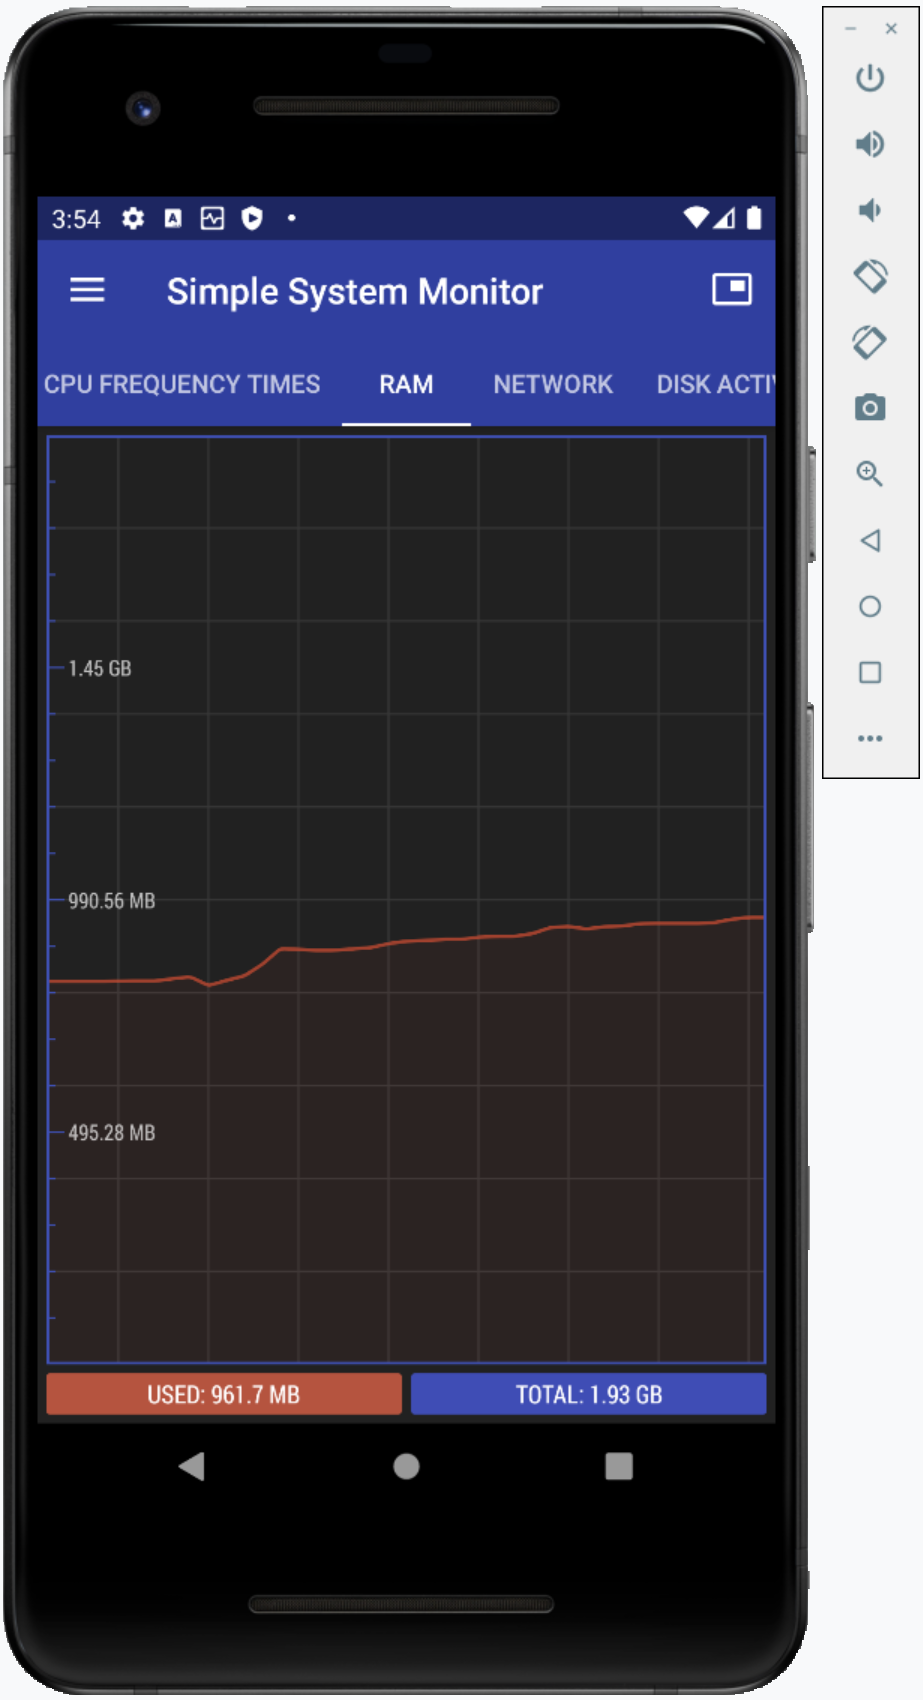
\includegraphics[width=4cm]{michael18.png}
\begin{minipage}{\linewidth}
\begin{wrapfigure}{l}{0.4\textwidth}
\centering
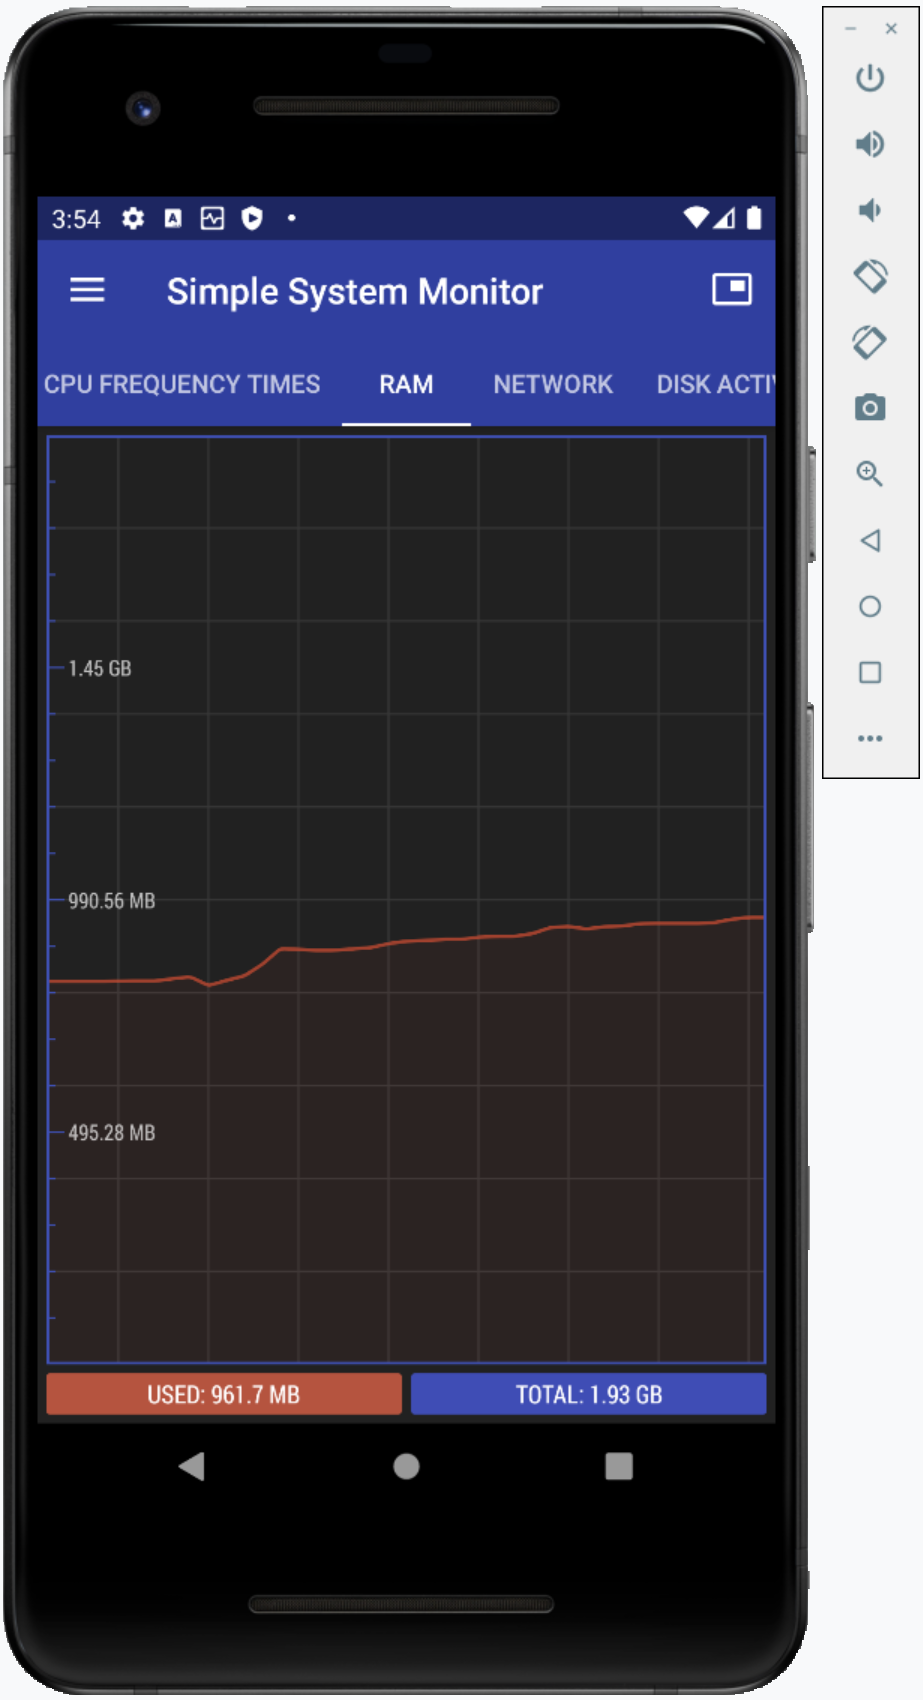
\includegraphics[scale=0.15]{michael18.png}
\end{wrapfigure}
~\\
~\\
~\\
~\\
~\\
~\\
~\\

This was the RAM benchmark of the malicious application. As can be seen, the data went up to about 960MB. Even after several tests, the malicious application used less RAM than the legitimate one. Why this one is more optimized than the real one is as of yet unknown, but perhaps it is possible to find the answer within the code after thorough searching. This version of the application used about 170MB of data. Which means a decrease to about 79% of the original.
\end{minipage}

\newpage
\subsection{Countermeasures and detection}

\subsubsection{Preventive measures}

The simplest way to avoid installing malicious apps would be to not download any APK files from the internet, instead using the Google Play Store, or alternatively for iPhone users the App Store. Even then, caution is advised. It is important to note what kind of permissions an application requires to install and run. A malicious application would most likely require more or unusual permissions. Another way of verifying the legitimacy of an application is to compare its hash or size, though size is not always a reliable measure, with one of a trusted source. Knowing what sources to trust is key to security in general. Keeping your phone or your phone’s software up to date is recommended as well. Lastly, since Android is open-source, the user is free to do whatever they desire with it. This causes complications for users who are not as well-versed in technology or phone software. Keeping users up to date with this kind of technology, and spreading awareness would reduce the amount of people who have been targeted by a huge amount.

\subsubsection{Detective measures}

There are two large indicators to identify the malicious application. The first being the mis-matched icons. Exceptional about this is that the app doesn’t need to be running to identify it. The second indicator is during start-up. If there is a message in Arabic which pops up, it is a fake application. Since this application is not all that dangerous, there is no harm in this. However, for other applications this method is not recommended: it could lead to an application running malicious code. Preventive measures still apply at this point, such as verifying the legitimacy of an app by hash or size, or by checking the source of the application.
\subsubsection{Reactive measures}

If the application is already installed it is recommended to remove it. Whatever the case, do not run the application. In the case of this app, uninstalling the software would work, but in other cases applications might be harder to remove or have installed additional malicious software. In that case it might be a good idea to restore a back-up. Both iOS and Android support and even recommend this feature, by use of iCloud or Google Drive. If the device becomes inaccessible, it might be necessary to run the device in safe mode. This way it could still be booted and the application could be removed.
\subsubsection{YARA rule set}

A simple way to filter this application is to create a YARA rule that detects if the string “www.farsroid.com” is present, and to specifically filter this app it is also useful to declare that the application size is below 40MB. Since the malicious version is smaller than the official one, and the official version is likely going to add updates such as extra levels or limited time events, the real app is likely to only get bigger. However, this condition could easily be removed so that the only requirement is that the string “www.farsroid.com” is present, to filter all apps made by this malicious developer.

\lstinputlisting[language=YARA]{individual/michael/ruleset1.yar}

Or alternatively the filter without the size requirement:

\lstinputlisting[language=YARA]{individual/michael/ruleset2.yar}

